\documentclass[9pt]{pnas-new}
\RequirePackage[slovene,english]{babel} % when writing in english
\templatetype{pnasresearcharticle} % Choose template 
\selectlanguage{english}


\usepackage{graphicx}
\usepackage{subfig}

\usepackage{hyperref}
\hypersetup{colorlinks=true,linkcolor=blue, linktocpage}

\usepackage{import}
\usepackage[subpreambles=true]{standalone}

% Fancy new commands
\newcommand{\set}[1]{\ensuremath{\mathbf{#1}}}
\renewcommand{\vec}[1]{\ensuremath{\mathbf{#1}}}
\newcommand{\uvec}[1]{\ensuremath{\hat{\vec{#1}}}}
\newcommand{\const}[1]{{\ensuremath{\kappa_\mathrm{#1}}}} 
\newcommand{\num}[1]{#1}

% Path settings
\graphicspath{{./figures/}}





















\title{Simulating flock of birds using only vision}

\author{Žiga Leskovec}
\author{Maksimiljan Vojvoda}
\affil{Collective behaviour course research seminar report} 
\leadauthor{Leskovec \& Vojvoda} 

\selectlanguage{english}

\significancestatement
{A model of collective behavior based purely on vision}
{
When modeling collective behaviour it is commonly assumed that agents inherently know other agents position, velocity and direction.
There exists a motivation to get rid of these assumptions and model the behaviour based on how internal and external information is acquired and processed.
Vision is one of the more important sensory systems that provide crucial external information, which turns out to be sufficient for modeling interactions between agents in a swarm.
In this seminar we explore a mathematical framework for perception-based interactions proposed by Renaud Bastien and Pawel Romanczuk.
}
{Simulation | Vision | Flock of birds }


% Please include corresponding author, author contribution and author declaration information
% \authorcontributions{Please provide details of author contributions here.}
%\authordeclaration{Please declare any conflict of interest here.}
%\equalauthors{\textsuperscript{1}A.O.(Author One) and A.T. (Author Two) contributed equally to this work (remove if not applicable).}
%\correspondingauthor{\textsuperscript{2}To whom correspondence should be addressed. E-mail: author.two\@email.com}

% Keywords are not mandatory, but authors are strongly encouraged to provide them. If provided, please include two to five keywords, separated by the pipe symbol, e.g:
\keywords{Simulation | Vision | Flock of birds }
\begin{abstract}
When modeling collective behaviour it is commonly assumed that agents inherently know other agents position, velocity and direction.
There exists a motivation to get rid of these assumptions and model the behaviour based on how internal and external information is acquired and processed.
Vision is one of the more important sensory systems that provide crucial external information, which turns out to be sufficient for modeling interactions between agents in a swarm.
In this seminar we explore a mathematical framework for perception-based interactions proposed by Renaud Bastien and Pawel Romanczuk.
\end{abstract}

\dates{\textbf{\today}}
\program{BM-RI}
\vol{2023/24}
\no{CB:F} % group ID
%\fraca{FRIteza/201516.130}

\begin{document}

% Optional adjustment to line up main text (after abstract) of first page with line numbers, when using both lineno and twocolumn options.
% You should only change this length when you've finalised the article contents.
\verticaladjustment{-2pt}

\maketitle
\thispagestyle{firststyle}
\ifthenelse{\boolean{shortarticle}}{\ifthenelse{\boolean{singlecolumn}}{\abscontentformatted}{\abscontent}}{}

\dropcap{M}odels of collective behaviour often rely on interactions that do not have a direct physical reality (such as neighbour velocity, relative position and direction).
One example of this is the simulation of fish schools \cite{wissel1992fish}.
However, this assumption of how the information is processed by agents limits our understanding of the underlying complexity that takes place in such phenomena.
A better alternative would be to model the behaviour around internal and external information that agents are capable of acquiring.

In this seminar we use a mathematical framework proposed by Renaud Bastien and Pawel Romanczuk \cite{main-paper}, to create a simulation of flock of birds that solely relies on vision.




























\section*{Methods}

The simulation is done in 2-dimensional space where agents are represented as simple disk objects with full $360^\circ$ view.
On each simulation step, their velocity is modified based on a projection of their surrounding visual field.
This simulates a primitive form of vision.



\subsection{Visual field projection}

\begin{figure}
    \centering
    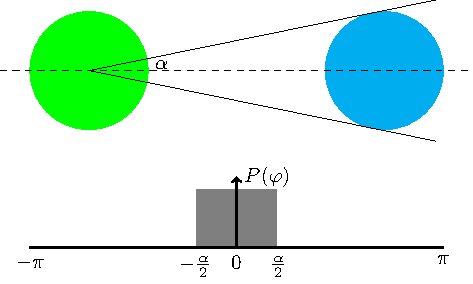
\includegraphics[width=0.9\linewidth]{projection.pdf}
    \caption{
       Projection field graph of a single object.
    }
    \label{fig:example-projection}
\end{figure}

\sloppy

Objects around the agent are projected onto their visual field, described by $P(\varphi)$.
Function $P(\varphi)$ represents visual obstructions of the agent, where $\varphi$ is an angle of the visual field. The result is binary, where 0 represents ``not obstructed'' and 1 represents ``obstructed''.
An example of a visual field projection can be seen on figure \ref{fig:example-projection}.

\fussy




\subsection{Velocity}

On each simulation step, the velocity of agent $i$, is modified by $\Delta v_i$.
The general speed delta is summarized with the following equation:

\begin{equation}
    \Delta v_i = \text{F}_{\text{ind}}(v_i) + \text{F}_{\text{vis}}(P_i)
\end{equation}

where $\text{F}_{\text{ind}}$ function represents speed delta collected from \textbf{ind}ividuals ``internal information'':

\begin{equation}
    \text{F}_{\text{ind}} = \gamma(v_\text{pref} - v_i)\hat{v_i}
\end{equation}

where $\gamma$ represents speed relaxation rate, $v_\text{pref}$ \textbf{pref}erred speed of the individual and $\hat{v_i}$ normalized direction vector.
Function $\text{F}_{\text{vis}}$ transforms \textbf{vis}ual field to the individuals speed delta.
It is independent of other individuals properties, and is described with the following equation:

\begin{equation}
    \text{F}_{\text{vis}}(P) = \int_{-\pi}^{\pi} \ G(P, \varphi) \ h(\varphi) \ d\varphi
\end{equation}

Here $G(P, \varphi)$ encodes how information from the visual field impacts the movement, while $h(\varphi)$ encodes properties of the perception-motor system, in our case, it describes how front-back distance impacts the speed and how left-right distance influences the heading direction of an agent.
For convenience the equation is split into two parts
\sloppy

\begin{equation}
    \Delta v_i = \gamma(v_\text{pref} - v_i) +
        \int_{-\pi}^{\pi} cos(\varphi) \ \alpha_0
        \left(
            -P_i(\varphi) \ + \ \alpha_1 (\partial_{\varphi} P_i(\varphi))^2
        \right) d\varphi
    \label{eq:speed}
\end{equation}


\begin{equation}
    \Delta \Psi_i =
        \int_{-\pi}^{\pi}
        sin(\varphi) \ \beta_0
        \left(
            -P_i(\varphi) \ + \ \beta_1 (\partial_{\varphi} P_i(\varphi))^2
        \right) d\varphi
    \label{eq:angle}
\end{equation}

The first ($\Delta v_i$) describes speed delta, while the second ($\Delta \Psi_i$) describes heading angle delta.
Consequently the heading vector is now removed, since it is encoded as the heading angle.

As we will see further in the seminar, parameters $\alpha_1$ and $\beta_1$ influence the equilibrium distances.
$\alpha_1$ influences the front-back distance equilibrium $\frac{r}{\alpha_1}$, while $\beta_1$ influences the left-right distance equilibrium $\frac{r}{\beta_1}$, where $r$ stands for agent radius.






\subsection{Integration of P}

One of the core elements of the simulation is calculating integrals of functions multiplied with $P$ such as $\int_{-\pi}^{\pi} cos(\varphi) P_i(\varphi)$ from equations \ref{eq:angle} and \ref{eq:speed}.
Because the projection function $P$ contains contiguous regions of values $0$ or $1$, we can split the integral into multiple definite integrals where we calculate only the sections where $P$ has value of $1$.
A visual representation of multiplying a trigonometric function with $P$ (in this case $cos$) can be seen on figure \ref{fig:integral}.
This trick trivialises the integral calculation.

\begin{figure}[h]
    \centering
    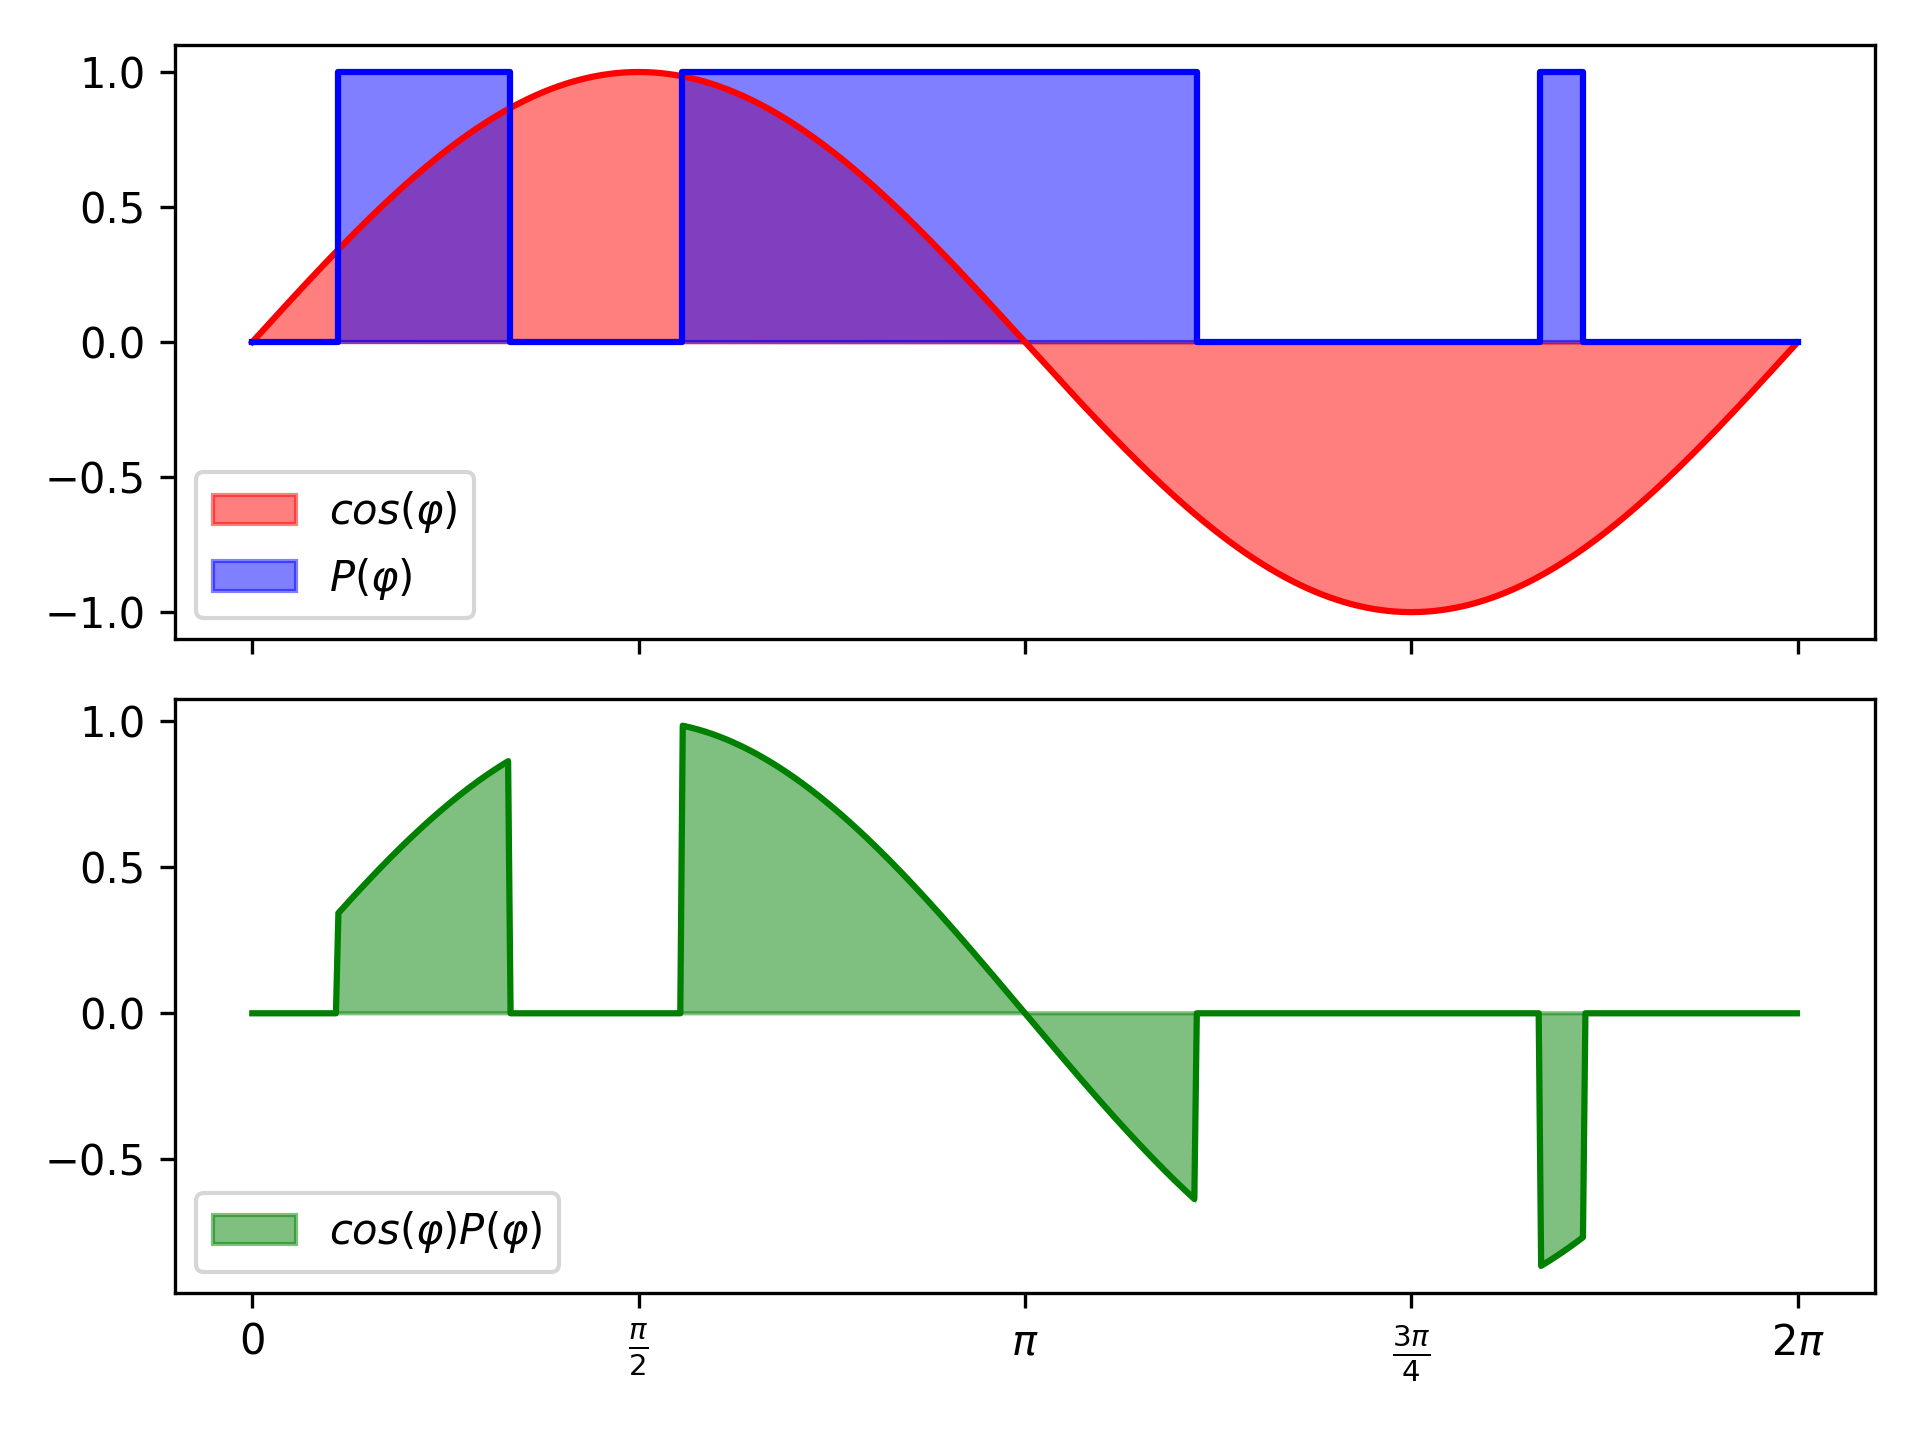
\includegraphics[width=\linewidth]{integral.png}
    \caption{
      Multiplying a function (in this case $cos$) with some projection function $P$.
    }
    \label{fig:integral}
\end{figure}




\subsection{Implementation}

The simulation is implemented in C++.

In the source paper \cite{main-paper}, the author calculates the projection function $P$ using ray casting.
We have improved on this by projecting the objects directly by calculating the appropriate angles of vision for each object as show in figure \ref{fig:example-projection}.
For each object we constructed an array of intervals where $P$ would have a value of $1$.
By carefully merging these intervals we kept the array \textit{clean} as none of the intervals would intersect.
With this array we could trivially calculate all the necessary components described in equations \ref{eq:speed} and \ref{eq:angle} using the method described in the previous section.


The underlying simulation loop is also parallelizable, as agents are dependant only on the previous state of the simulation, therefore we can use multi-threading to increase the simulation speed, thus allowing us to simulate larger or longer simulations.







\subsection{Simulation visualisation}

% Visualisation of the simulation will be done using FFmpeg\footnote{\url{https://ffmpeg.org/}}, which will encode an array of pixels (representing a state of the simulation) into an image or a video.
The speed of image generation is not important to this seminar and is therefore done separately in Python with Matplotlib.
Every simulation figure has its own one minute long animation available on our Github repository \url{https://github.com/siggsy/collective-vision/tree/main/results}.
It is worth noting that the size of the agents is not to scale.


\section*{Results}

Every simulation was run for 2000 steps with 50 agents randomly placed in a box bounded by $(0,0)$ and $(5,5)$.
All agents had a radius of $0.5$ and had $v_\text{pref}$ set to $0.5$.
Simulation parameters were set to the following values:
\begin{enumerate}[label=$\bullet$]
    \item $\alpha_1 = 0.08$
    \item $\beta_1 = 0.08$
    \item $\gamma = 0.95$
\end{enumerate}

In figure \ref{fig:simulation} we can see 3 different collective behaviours using $\alpha_0$ and $\beta_0$ parameters found in the paper this seminar is based on\cite{main-paper}.

\begin{figure}[H]
    \centering
    \begin{tabular}{cc}
        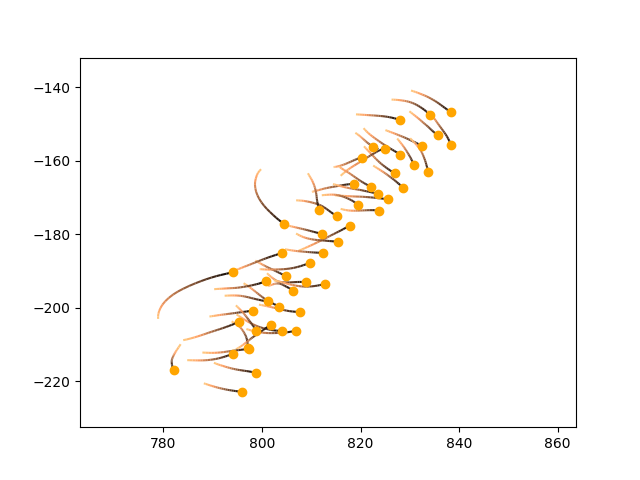
\includegraphics[width=0.47\textwidth]{line.png} &
        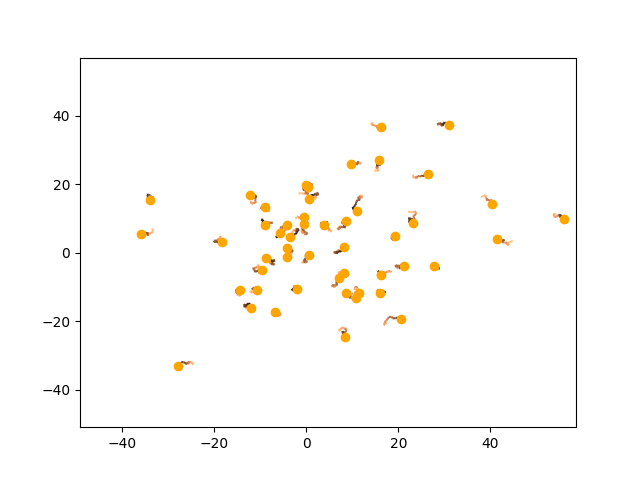
\includegraphics[width=0.47\textwidth]{crystal.png} \\
        (a) Polarized line ($\alpha_0 = 0.5$, $\beta_0 = 0.01$) & (b) Crystal ($\alpha_0 = 0.1$, $\beta_0 = 10$) \\
        \multicolumn{2}{c}{
            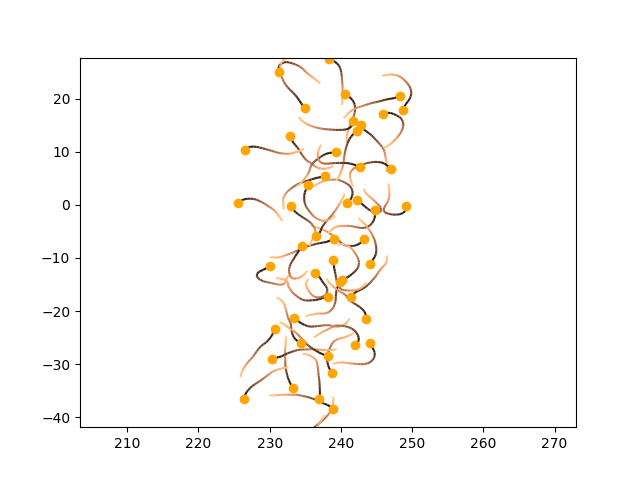
\includegraphics[width=0.5\textwidth]{swarm.png}
        } \\
        \multicolumn{2}{c}{(c) Swarm ($\alpha_0 = 0.5$, $\beta_0 = 1$)}
    \end{tabular}
    \caption{Last frames of the tested simulations}
    \label{fig:simulation}
\end{figure}

In simulation (a) all agents move in one general direction and form a line.
In contrast, in simulation (b) agents shake in-place and barely make any distance.
Since the figures represent the last frames of the animation, this can be observed by checking their final coordinates.
In the final simulation (c) agents are moving around freely while maintaining a swarm.




% Uporabljamo višinske karte velikosti 512$\times$512 točk. Začetni teren se, predvsem zato ker je opravilo prepuščeno centralni procesni enoti, v povprečju zgradi v 3\,s. Ker se ta korak izvede samo enkrat v celotnem procesu to ni moteče. Nadaljna simulacija naravnih procesov se izvaja hitro; s frekvenco 94\,Hz (iteracij na sekundo), ko se izvaja zgolj proces hidravlične erozije, 108\,Hz, ko se izvaja zgolj proces termične erozije, in 85\,Hz, ko se izvajata oba procesa erozije sočasno. Simulacije rasti koralnega grebena ne izvajamo sočasno z erozijo, ampak ločeno, ta se izvaja s frekvenco 108\,Hz. Najhitrejša je vizualizacija, ki takrat, ko se ne izvaja nobena simulacija, dosega prikaz z 124\,fps (slik na sekundo). V celoti generiranje otoka želenega videza traja od 10 do 15 sekund. Vse vrednosti veljajo za prenosni računalnik s procesorjem Intel Core i7 4700-HQ, 8\,GB delovnega pomnilnika in grafično kartico nVidia GTX 760M, pri čemer smo v pogonu Unity 5 imeli nastavljen prikaz z najvišjo stopnjo podrobnosti.

% Predstavljen postopek torej uspešno generira začetni teren, na katerem simulira hidravlično in termično erozijo ter nato še rast koralnega grebena. Končni teren z nanesenimi teksturami in izrisom morske gladine ima prepričljiv videz tropskega otoka. S spreminjanjem parametrov lahko dobimo veliko različnih oblik otoka, kot prikazujeta primera na sliki \ref{fig:final_island_1}.

% Z videzom tropskega otoka smo zadovoljni, hidravlična in termična erozija skupaj oblikujeta razgiban teren brez večjih vidnih napak. Dodan korak difuzije sedimenta se dobro obnese, vendar ni fizično natančen. Transport sedimenta in logika nalaganja sedimenta potrebujeta še nekaj izboljšav. Težava modela hidravlične erozije je v tem, da je težko uravnovesiti vse konstante v simulaciji. Simulacija hitro postane nestabilna, kar povzroča večje napake na terenu. Maške \cite{maske_2013} je v svojem diplomskem delu dosegel boljši transport in nalaganje sedimenta. Hitrosti izvajanja pa zaradi uporabe različne strojne opreme ne moremo primerjati z njegovo.

% Simulacija rasti koralnega grebena daje prepričljive rezultate in se izvaja hitro. Videz grebena bi lahko bil bolj razgiban, saj se trenutno ob obali otoka ustvari popoln in neprekinjen greben. Naravni grebeni so mnogokrat prekinjeni in različno oddaljeni od obale. Tako kot pri hidravlični eroziji smo tudi v primeru simulacije rasti koralnega grebena imeli težave z uravnovešanjem konstant, saj ima že zelo majhna sprememba velik vpliv na končni rezultat.

% Dinamično nanašanje tekstur deluje hitro in daje prepričljiv videz. Vzorčne teksture lahko zamenjamo in tako na preprost način spremenimo videz otoka. Videz otoka lahko spreminjamo tudi s spreminjanjem parametrov v senčilniku, kot sta na primer gostota ponavljanja posamezne vzorčne teksture in naklon terena, pri katerem namesto teksture trave nanesemo teksturo skale. 

% Gladina morja veliko pripomore k prepričljivosti vizualizacije otoka. Senčilnik se dobro obnese, saj nam daje tudi vizualno informacijo o globini vode, kar je še posebno koristno v okolici koralnega grebena. Prikaz sicer ni fizikalno natančen, saj zanemari kot pogleda. Globino vedno izrisuje, kot da je pogled od zgoraj navzdol. V praksi pa to ne povzroča težav, saj teren večino časa opazujemo iz zraka.







































\section*{Discussion}

In this seminar we implemented and simulated a collective behaviour of birds using only their vision.
We have improved on the original work by Bastien and Romanczuk \cite{main-paper} by replacing ray casting with direct projection.
This improved the accuracy and calculation efficiency of the visual fields of the birds.

The simulation is limited to only 2 dimensions as visualisation of more would be quite cumbersome. 

% V delu smo predstavili postopek, ki na podlagi vhodnih parametrov generira teren v obliki otoka, na katerem v realnem času nato simulira hidravlično in termično erozijo ter za tem še rast koralnega grebena. Na teren dinamično nanaša teksture in izrisuje gladino morja. Zadani cilj, da ima generiran teren prepričljiv videz tropskega otoka z okoliškim koralnim grebenom, smo po našem mnenju dosegli. 

% Končni teren je uporaben predvsem v strateških igrah, kjer nanj večinoma gledamo iz oddaljenosti. Teren namreč nima dovolj podrobnosti za prvo osebne igre, kjer se igralec po terenu sprehaja  in ga raziskuje. Čas potreben za generiranje otoka želenega videza je pri uporabi v računalniški igri
% %, katere namen ni dinamično spreminjanje terena, 
% lahko težava, vendar bi jo z izboljšanjem implementacije lahko odpravili. Generiranje začetnega terena bi lahko pospešili tako, da bi ga namesto v jeziku C\# implementirali v nižjenivojskem jeziku (npr. C++) ali pa na senčilniku. Hitrost izvajanja simulacij naravnih procesov na GPE bi lahko optimizirali, saj se v trenutni implementaciji opravlja nepotrebno kopiranje tekstur, kar izvajanja simulacij upočasni. 

% Terenu bi lahko dodatno izboljšali videz s tem, da bi za njegovo predstavitev uporabili več plasti z različnimi trdotami, kar bi morali nato upoštevati tudi pri simulacijah procesa erozije \cite{benevs_layered_08}. Funkcije, ki generirajo začetni teren, pa smo že zasnovali tako, da lahko izhod ene uporabimo kot vhod druge. S tem imamo več možnosti pri gradnji začetnega terena; nismo omejeni zgolj na obliko stožca. 























\acknow{Žiga Leskovec fine tuned the simulation parameters and handled the simulation visualisation; Maksimiljan Vojvoda implemented the simulation loop.}
\showacknow % Display the acknowledgments section

% \pnasbreak splits and balances the columns before the references.
% If you see unexpected formatting errors, try commenting out this line
% as it can run into problems with floats and footnotes on the final page.
%\pnasbreak

\begin{multicols}{2}
\section*{\bibname}
% Bibliography
\bibliography{./bibliography}
\end{multicols}

\end{document}